\documentclass{report}
\usepackage{graphicx} % Required for inserting images
\usepackage[italian]{babel}
\usepackage{tikz}
\usepackage{hyperref}
\usepackage{amsmath}
\usepackage{xcolor}
\usepackage{float}
\usepackage{soul}
\usepackage{listings} % Per evidenziare il codice

\definecolor{lightgray}{rgb}{0.9,0.9,0.9} % Definizione colore sfondo
\definecolor{darkgreen}{rgb}{0.0, 0.5, 0.0}

\lstset{
    backgroundcolor=\color{lightgray}, % Sfondo grigio
    basicstyle=\ttfamily, % Font monospaziato
    % frame=single, % Bordo attorno al codice
    tabsize=4, % Dimensione tabulazione
    breaklines=true, % Permette di andare a capo automaticamente
    numbers = left,
    numberstyle=\small\color{gray}
}

\title{\huge\textbf{{Controllo degli Accessi}}}
\date{Parte I}

\begin{document}

\maketitle

\tableofcontents
\newpage

\chapter{Introduzione}

\noindent Il \textbf{controllo degli accessi} valuta l'accesso richiesto alle risorse dagli 
utenti autenticati e, sulla base di \textit{regole di accesso} (definite all'interno)
del sistema, determina se l'accesso sia garantito o negato.

Si occupa solamente dell'\textbf{accesso diretto}. Si basa su due concetti:
\begin{itemize}
    \item \textbf{Autenticazione/Identificazione} dell'utente che fa la richiesta
    \begin{itemize}
        \item importante anche per le problematiche di \textit{accountability}; posso
        analizzare i log per capire chi ha fatto che cosa nel caso ci sia un problema
    \end{itemize}
    \item \textbf{Correttezza delle autorizzazioni} con cui l'accesso viene valutato
\end{itemize}

\section{Politiche, modelli, meccanismi}
È utile fare una distinzione tra:
\begin{itemize}
    \item \textbf{Politiche:} sono i requisiti di protezione ad alto livello che voglio applicare 
    al mio sistema 
    \item \textbf{Model:} viene usato per rappresentare la politica 
    \item \textbf{Meccanismi:} implementano la politica con \textit{hw} e \textit{sw}
\end{itemize}

\noindent Risulta utile fare questa distinzione perché comporta dei vantaggi: posso 
verificare se il modello è corretto rispetto alla politica che ho definito; lo 
stesso meccanismo può essere usato per implementare politiche o modelli diversi.

\subsection{Meccanismo}
In letteratura prende il nome di \textit{reference monitor}, deve soddisfarre le 
seguenti proprietà:
\begin{itemize}
    \item non può essere modificabile; nel caso in cui venga fatto me ne devo accorgere 
    \item non può essere bypassabile 
    \item deve essere confinato ad una specifica parte del mio sistema (non distribuito)
    \item deve essere abbastanza piccolo per essere soggetto a processi di verifica formale
\end{itemize}

\noindent Il meccanismo deve essere sicuro rispetto ai canali di comunicazione non 
legittimi:
\begin{itemize}
    \item \textbf{Storage channels:} le parti di memoria, prima di essere rese disponibili 
    ad altri dati, dovrebbero essere \textit{pulite} (se cancello un dato non è che \textit{sparisce} dalla 
    memoria fisica dal computer \dots)
    \item \textbf{Covert channels:} canali non intesi per il trasferimento di informazioni
    che possono essere usati per inferire informazioni
\end{itemize}

\subsubsection{Alcuni principi di design}
\begin{itemize}
    \item \textit{Separazione dei privilegi:} non dare troppo \textit{potere} ad un solo utente 
    \item \textit{Privilegio minimo:} voglio darti il minimo privilegio di cui hai bisogno
\end{itemize}

\section{Processo di sviluppo di un AC}
Una volta definito il modello, posso verificare due aspetti:
\begin{itemize}
    \item \textbf{Completezza:} verificare che hai rappresentato tutti i requisiti di sicurezza della politica
    \item \textbf{Consistenza:} dev essere privo di contraddizioni (un utente ha sia accesso/negazione per una risorsa)
\end{itemize}






\chapter{Discretionary (DAC) policies: approcci base}

\noindent Sono politiche basate su:
\begin{itemize}
    \item \textbf{identità} degli utenti 
    \item definizione di regole di accesso (\textbf{autorizzazioni}), che stabiliscono
    \textit{chi può fare che cosa}
\end{itemize}

\noindent Definite \textit{discrezionale} perché gli utenti che sono proprietari 
dei dati possono amministrarli come vogliono, \textit{a loro discrezione}; tipicamente, 
non ho un unico amminstratore, ma ci sono più amministratori proprietari delle risorse: è 
in mano a qualcuno stabilire chi può accedere o meno alle risorse (non è escluso avere 
un unico amministratore).

\section{Un esempio di modello}
Si usa la \textit{matrice degli accessi}, è una rappresentazione astratta della 
politica di protezione del sistema.

\noindent Formalmente, è caratterizzato da una tripla $(S, O, A)$ che rappresenta 
lo stato del sistema, dove:
\begin{itemize}
    \item $S$ è il set degli utenti 
    \item $O$ è il set delle risorse, dove $S \subset O$ (un soggetto può essere anche un processo, e può 
    essere anche una risorsa \dots)
    \item $A$ è la matrice, dove:
    \begin{itemize}
        \item le righe corrispondono ai soggetti 
        \item le colonne corrispondono agli oggetti 
        \item $A[s, o]$ riporta i privilegi di $s$ su $o$
    \end{itemize}
\end{itemize}

\begin{figure}[H]
    \centering
    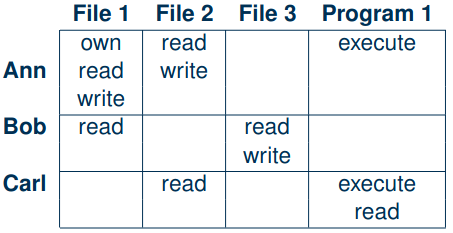
\includegraphics[width=0.6\linewidth]{images/dac1.png}
\end{figure}

\noindent I cambi di stato del sistema vengono fatti con dei comandi che chiamano delle \textbf{operazioni primitive}:
\begin{itemize}
    \item \texttt{enter} $r$ into $A[s,o]$
    \item \texttt{delete} $r$ from $A[s,o]$
    \item \texttt{create} subject $s$
    \item \dots
\end{itemize}

\noindent Sono della forma:

\begin{figure}[H]
    \centering
    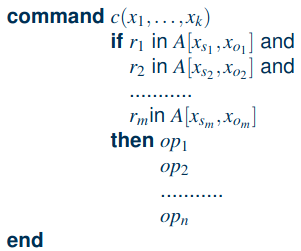
\includegraphics[width=0.45\linewidth]{images/dac-comm.png}
\end{figure}

\noindent Un esempio:

\begin{figure}[H]
    \centering
    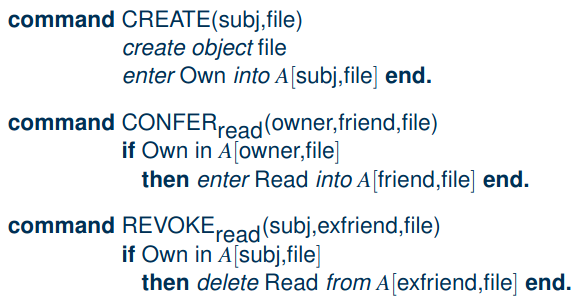
\includegraphics[width=0.65\linewidth]{images/dac2.png}
\end{figure}

\section{Trasferimento dei privilegi}
Il proprietario dei dati può dare il privilegio anche ad altri utenti.
Può rappresentato in modo formale in due modi differenti:
\begin{itemize}
    \item \textbf{Copy flag (*):} il soggetto trasferisce il privilegio ad altri; mantiene il privilegio
    \begin{figure}[H]
        \centering
        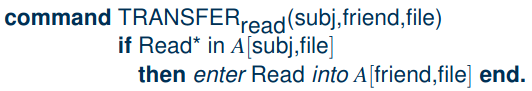
\includegraphics[width=0.6\linewidth]{images/transfer1.png}
    \end{figure}
    \item \textbf{Transfer-only flag(+):} il soggetto trasferisce ad altri il privilegio ma perde l'autorizzazione
    \begin{figure}[H]
        \centering
        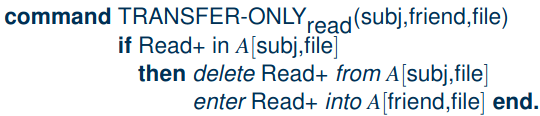
\includegraphics[width=0.6\linewidth]{images/transfer2.png}
    \end{figure}
\end{itemize}

\noindent Partendo da uno stato \textit{sicuro}, non deve accadere che applicando una o più operazioni 
si finisca in uno stato non sicuro.

\section{Implementazione della matrice}
La matrice è spesso sparsa, salvarla sarebbe uno spreco di memoria. Ci sono diversi 
approcci alternativi:
\begin{itemize}
    \item \textbf{Tabella di autorizzazione}; tabella di tuple $(S, O, A)$ non nulle
    \begin{figure}[H]
        \centering
        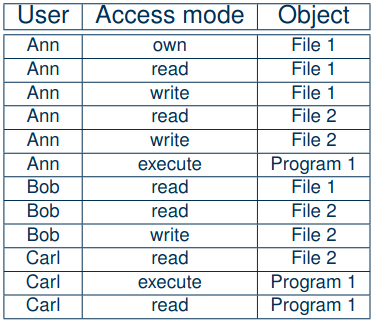
\includegraphics[width=0.5\linewidth]{images/auth-table.png}
    \end{figure}
    \newpage
    \item \textbf{Access Control Lists (ACLs)}: store by column; ad ogni risorsa associo una lista 
    che mi dice gli utenti quali operazioni possono fare
    \begin{figure}[H]
        \centering
        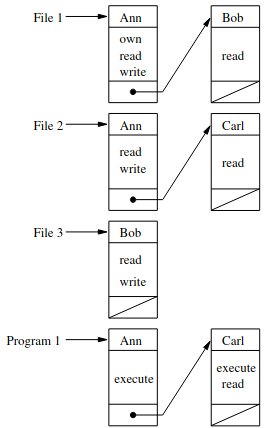
\includegraphics[width=0.4\linewidth]{images/acl.png}
    \end{figure}
    \item \textit{Capability lists}; store by row; sono come le precedenti ma vengono fatti storando per utenti
    invece che per risorse. Sono state soppraffatte dalle ACLs
    \begin{figure}[H]
        \centering
        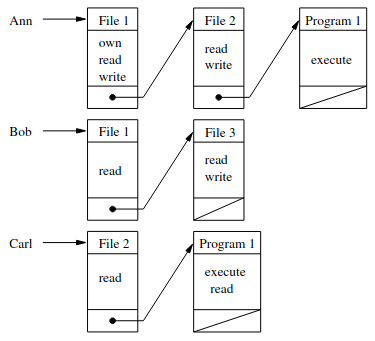
\includegraphics[width=0.5\linewidth]{images/capability.png}
    \end{figure}
\end{itemize}

\subsubsection{ACLs vs Capability lists}
\begin{itemize}
    \item non richiedono 
    autenticazione del soggetto, ma richiedono la possibilità di verificare che non siano state impropriamente 
    modificate \dots difficile da verificare (per questo non hanno avuto grande successo)
    \item le ACLs funzionano meglio quando fare delle operazioni di revoca per oggetto (ovviamente viceversa se devo fare revoche per soggetto)
\end{itemize}

\section{Debolezze di DAC}
Consentono il controllo solo sull'accesso \textbf{diretto}. Sono vulnerabili ai \textit{trojan 
horses}, ovvero accessi indiretti.

\begin{figure}[H]
    \centering
    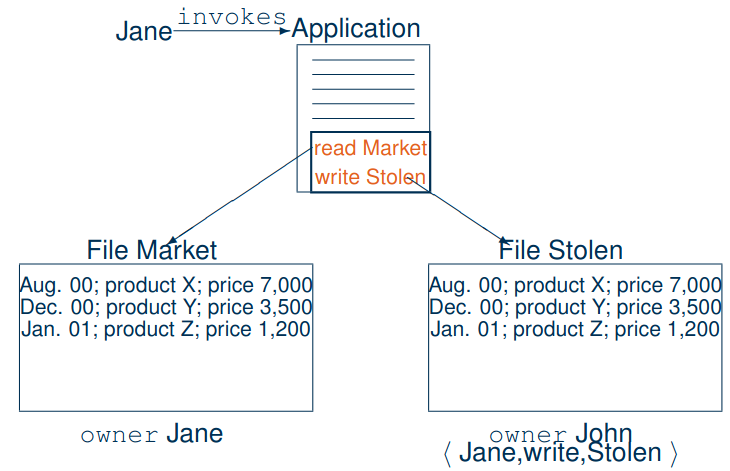
\includegraphics[width=0.8\linewidth]{images/trojan.png}
\end{figure}

\noindent L'idea è che vengono lasciate delle \textit{operazioni nascoste} in una applicazione per 
poter fare delle operazioni che normalmente non si avrebbe l'autorizzazioni di fare.

$\rightarrow$ è un accesso indiretto; è il processo che Jane sta eseguendo a chiedere l'accesso ai file



\chapter{Mandatory (MAC) policies}
\noindent Partono dall'assunzione che c'è una differenza tra \textit{utente} e \textit{soggetto}; è ciò 
che serve per bloccare i \textit{trojan horses}:
\begin{itemize}
    \item \textbf{Utente:} essere umano (di cui mi fido)
    \item \textbf{Soggetto:} processo nel sistema; opera per conto dell'utente; \textbf{non sono fidati} 
\end{itemize}

\noindent La politica più comune sono quelle \textbf{multilivello}: ogni soggetto e 
oggetto sono classificate con una etichetta. Si differenziano in politiche che si focalizzano su:
\begin{itemize}
    \item confidenzialità (Bell La Padula)
\end{itemize}

\textit{oppure}

\begin{itemize}
    \item integrità (Biba)
\end{itemize}

\section{Classificazione di sicurezza}
Ogni soggetto ed oggetto è associato ad una coppia di elementi:
\begin{itemize}
    \item \textbf{Livello di sicurezza:} livelli su cui è definita una relazione d'ordine totale (li posso mettere \textit{in fila}).
    \begin{center}
        $Secret > Confidential > Unclassified$
    \end{center}
    \item \textbf{Categoria:} insieme di elementi su cui non è definita alcuna relazione di ordinamento; serve 
    per partizionare aree differenti del sistema. Ad esempio, l'università ha un sacco di informazioni di vario 
    tipo: anagrafiche, finanziare, accademiche, \dots. 
    
    \noindent Hanno l'obiettivo di classificarle in classi diverse. Viene fatta 
    sia lato oggetto che lato soggetto.
\end{itemize}

\noindent La combinazione di queste due permette di definire una \textbf{relazione di dominanza:}
\begin{center}
    $(L_1, C_1) \geq (L_2, C_2) \Leftrightarrow L_1 \geq L_2 \land C_1 \supseteq C_2$
\end{center}

Questa relazione soddisfa una serie di proprietà che, in matematica, permette di formare 
un \textit{reticolo} (quando combinata fra tutte le classi); nel nostro caso parliamo 
di \textbf{reticolo di classificazione}.

\begin{figure}[H]
    \centering
    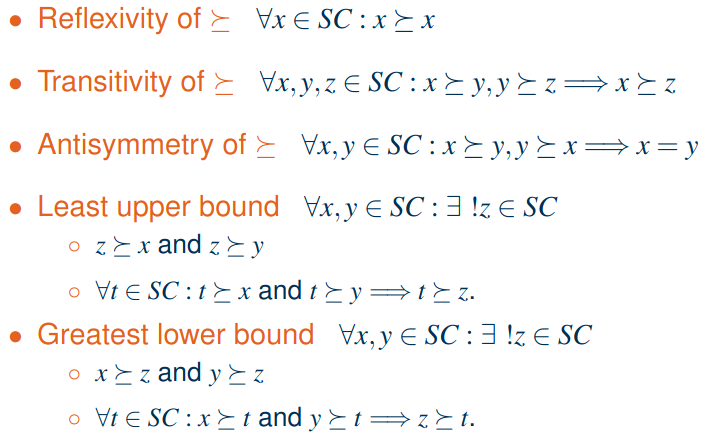
\includegraphics[width=0.8\linewidth]{images/props.png}
\end{figure}

\noindent Esempio di reticolo di classificazione:
\begin{figure}[H]
    \centering
    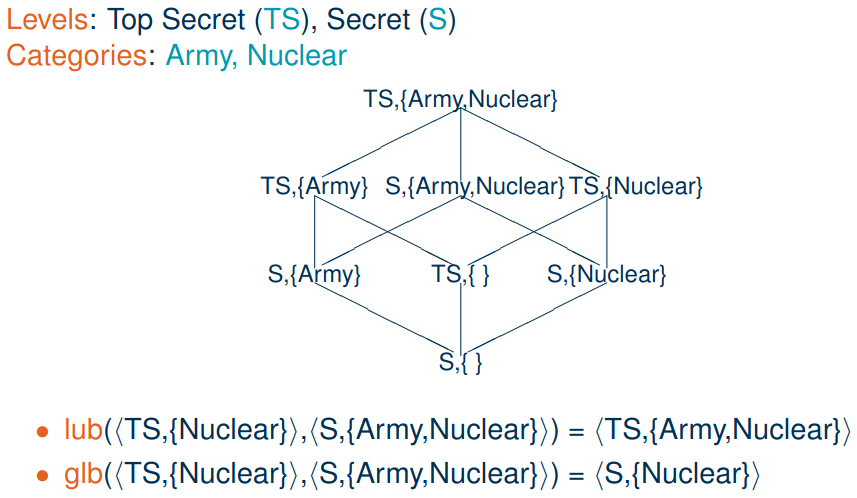
\includegraphics[width=0.8\linewidth]{images/reticolo.png}
\end{figure}

\newpage
\section{Semantica della classificazione di sicurezza}
\begin{itemize}
    \item \textbf{Classi di sicurezza}
    \begin{itemize}
        \item associato ad un \textit{soggetto}, rilfette la fiducia verso quell'utente; quanto mi fido di quell'utente 
        \item associato ad un \textit{oggetto}, riflette la sensisibilità dell'informazione
    \end{itemize}
    \item Le \textbf{categorie} definiscono l'area di competenza di utenti e dati.
\end{itemize}

\section{Bell La Padula}
È un modello che si preoccupa della confidenzialità (e non del resto).

\noindent Considerando di essere in un ambiente multilivello, l'\textbf{obiettivo} è 
prevenire flussi di informazioni ai livelli più bassi o a classi incomparabili.

\begin{itemize}
    \item \textbf{\textit{Simple property:}} un soggetto $s$ può leggere un oggetto 
    $o$ solo se $\lambda(s) \geq \lambda(o)$
    \item \textbf{\textit{*-property:}} un soggetto $s$ può scrivere un oggetto $o$ solo 
    se $\lambda(o) \geq \lambda(s)$
\end{itemize}

$\Rightarrow$ \textbf{NO READ UP}

$\Rightarrow$ \textbf{NO WRITE DOWN}

\noindent \textit{Se sono Secret, e scrivo un file secret in uno Top-Secret, non è mica un problema 
per la confidenzialità. Potrebbe esserlo se scrivo secret in un file Unclassified (potrebbe causare problemi a livelli di integrità, ma ci stiamo occupando solo di confidenzialità).}





\end{document}